\chapter[Introduction]{Introduction}
\label{Chap:Intro}

% ***************************************************
% Introduction
% ***************************************************

\section{Background and motivation}

\subsection{Overview of cellular communication in cancer}
Cell-cell communication is a mechanism that enables one cell to influence the behaviour of itself or another cell to ultimately coordinate biological processes to respond to the changes in intracellular and extracellular environments. It is vital for individual cells to be able to communicate with each other and their environment as a part of a functional multicellular organism to enable higher-order biological processes. For example, during embryonic development, cells differentiate into complex tissues and organs and these fate decisions are controlled through communications between neighbouring cells \cite{gale1996eph, eichmann1997ligand}. Responses of immune cells against pathogens or tumour cells are another example of cell-cell communication. When these signals are missing (e.g. in vitro), certain cell types enter a suicide program known as apoptosis (Figure \ref{fig:Chap1_figure1}). 

By studying cell communication, we can systematically understand coordinated cellular behaviours and unravel complex extracellular responses. Cell behaviours that consist of different complex processes are governed by specific combinations of extracellular signals (multiple ligands) rather than a single signal alone (Figure \ref{fig:Chap1_figure1}A-C). Each cell has been programmed to respond to a specific set of extracellular signals to survive and perform specialised functions. Each cell often requires multiple signals to survive (Figure \ref{fig:Chap1_figure1}A) or grow and divide (Figure \ref{fig:Chap1_figure1}B). Some signals can induce changes in cells' outward behaviours or appearance such as cell differentiation (Figure \ref{fig:Chap1_figure1}C). If deprived of appropriate survival signals, a normal cell will activate the apoptosis process (Figure \ref{fig:Chap1_figure1}D). The mechanisms behind cell communication commonly involve the combinations of extracellular proteins called ligands and transmembrane proteins called receptors \cite{alberts2018molecular}. Even with the same set of signals, distinct cell types can respond differently as the responses of the cells also rely on the combination of receptor proteins they possess. There are thousands of ligand-receptor pairs that have been curated over the last decade \cite{salwinski2004database, orchard2012protein} and the number of signalling combinations and responses are almost infinite.

\begin{figure}[htp]
% \renewcommand{\figurename}{Supplementary Figure}
    \centering
    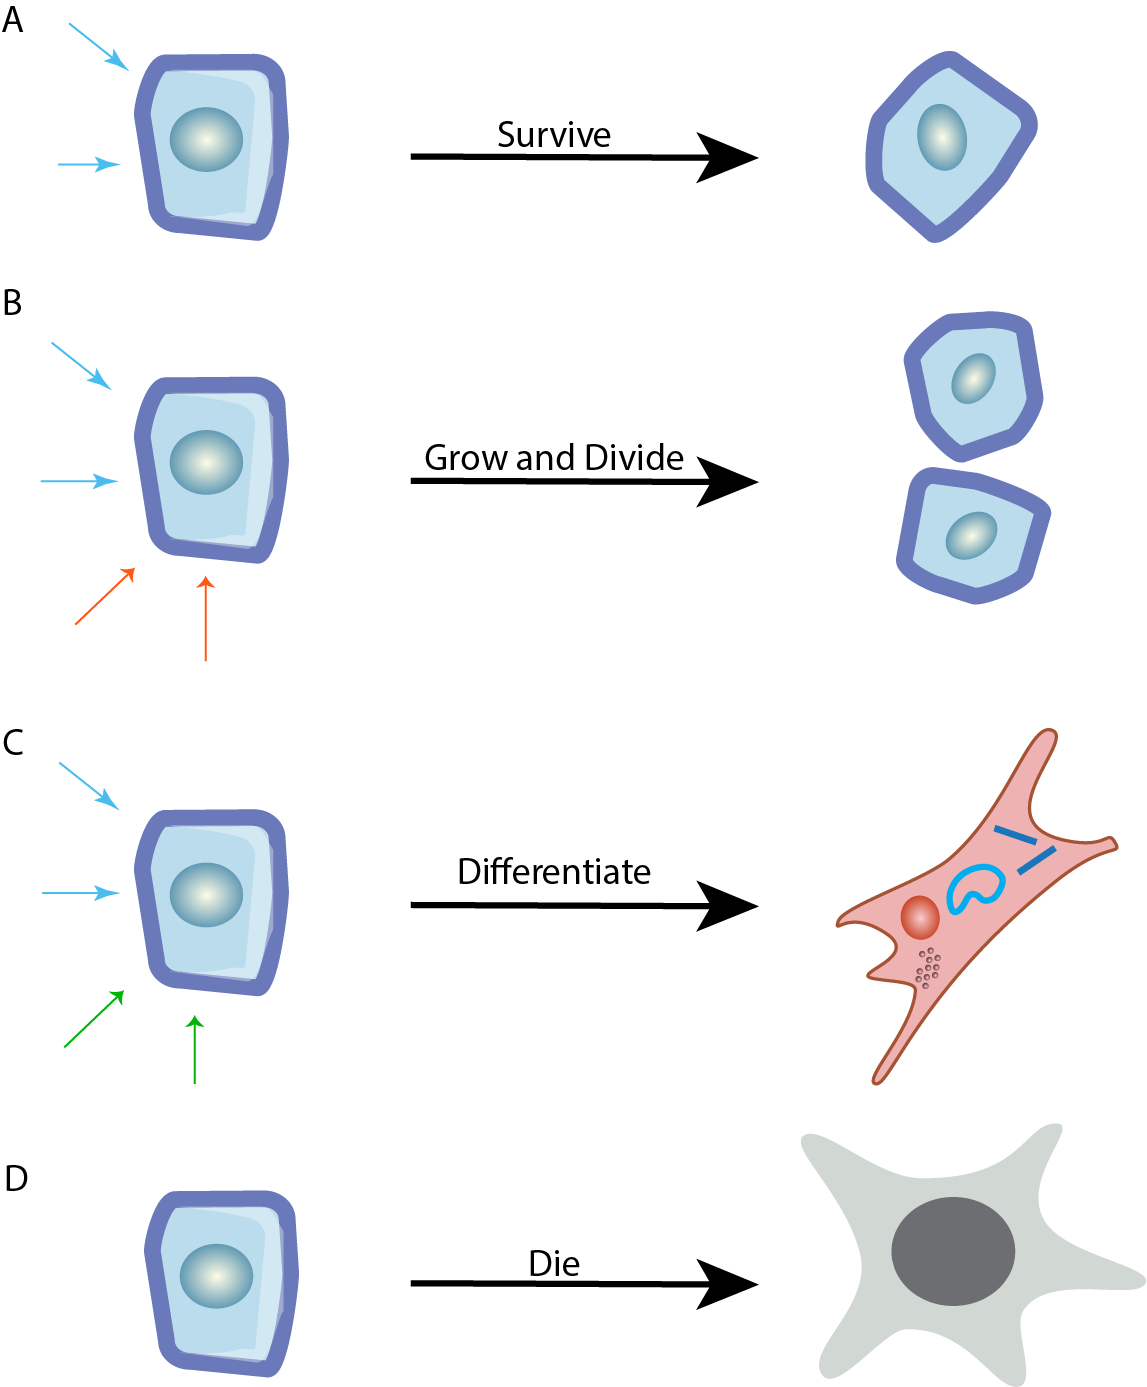
\includegraphics[width=0.6\columnwidth]{Chapter1/Figures/Chap1_figure1.png}
    \caption[Cell relies on multiple extracellular signalling molecules to survive.]{A cell can receive and respond to the signalling molecules produced by other cells using a set of receptors. The behaviours of a cell vary depending on the type of signals including to (A) survive (blue arrows), (B) grow and divide (red arrows) or (C) differentiate (green arrows). (D) The absence of survival signals can induce the cell suicide program known as apoptosis}
    \label{fig:Chap1_figure1}
\end{figure}

It is natural to make an analogy between the cell signalling systems and a human social organisation. The organisation relies on collaboration and coordination from multiple departments to operate functionally. The well-being of the individual is often set to lower the benefit of the whole. Similarly, cells in multicellular organisms heavily rely on the interaction between individuals to be functional \cite{bartee2018principles}. Through advances in computational biology and experimental throughput, we can now intensively characterise these signalling mechanisms and even simulate the cell-cell signalling networks to better understand the principles of how the interactions between cells can drive biological function \cite{sprinzak2010cis, teague2016synthetic, toda2019engineering}. Furthermore, technology development enables us to conduct more experiments in cells within living organisms \cite{helmchen2005deep, periasamy2013methods}, and spawns new means to study the cell microenvironment within a tissue context. 

Before discussing the approaches to studying cell-cell interaction in their spatial proximity, it is reasonable to revisit the major types of communications the cells can perform. To perform the communication, the cell secretes signalling molecules outside of the cell's membrane. The molecules can transmit through short or long distances and bind to the receptors at the surface of the target cell's membrane. Some signalling molecules are so small and unstable that require two cell membranes to be in contact to exchange signals. However, in most cases, the signalling molecules can travel to distant cells in which the gradient of factor received can determine the behaviours.         

The interaction between cells, in which two cells are physically in contact, is called \textit{gap junctions}. These are specialized intercellular connections that link the cytoplasm of two adjacent cells via narrow-filled channels (Figure \ref{fig:Chap1_figure2}A). The channels allow cells to exchange various small molecules, and ions but not macro-molecules, such as proteins or nucleic acids. Studies show that communication through gap junctions plays crucial roles in cell synchronization, differentiation, embryonic development, and immune response \cite{white1999genetic, vinken2006connexins}. For example, severe defects in heart development were found in mouse embryos to be caused by the mutation of one particular gap-junction protein (connexin 43)

While gap junctions are contact-dependent communications and allow cells to exchange ions or second messengers, cell communication also can take place across near or long distances. In most cases, signalling molecules are secreted to the outside of the membrane of signalling cells which act as local mediators, affecting neighbouring cells in the immediate environment. Alternatively, the signalling molecules can also transmit through the circulation to act on target cells at far distant sites \cite{cooper2004cell, alberts2018molecular}. The former signalling pathway when molecules are transmitted via a local distance is called \textit{paracrine signalling}. In paracrine signalling, cells secrete signalling molecules called ligands and induce changes in nearby cells (Figure \ref{fig:Chap1_figure2}B). The ligand molecules in paracrine signalling tend to be rapidly absorbed by neighbouring target cells; destroyed by extracellular enzymes, or immobilized by the extracellular matrix. Prominent examples of paracrine signalling systems include neurotransmitters between nerve cells at a synapse,  blood clotting system, tissue repair, and formation of scars
\cite{huang1998gap}. 

The alternative form of distant signalling is when the molecules travel through the extracellular fluids to reach receiver cells called \textit{endocrine signalling}. Endocrine cells secrete their signalling molecules in the form of hormones, into the blood circulation, which sends the signal to targets cell throughout the body (Figure \ref{fig:Chap1_figure2}C). Signal transmission in endocrine systems is much slower than in paracrine signalling and tends to last for long as it relies on diffusion and blood flow. One classic example is pancreatic cells producing the hormone insulin which signals cells in fat, muscles, and liver to absorb glucose and maintain blood sugar levels.

\begin{figure}[htp]
% \renewcommand{\figurename}{Supplementary Figure}
    \centering
    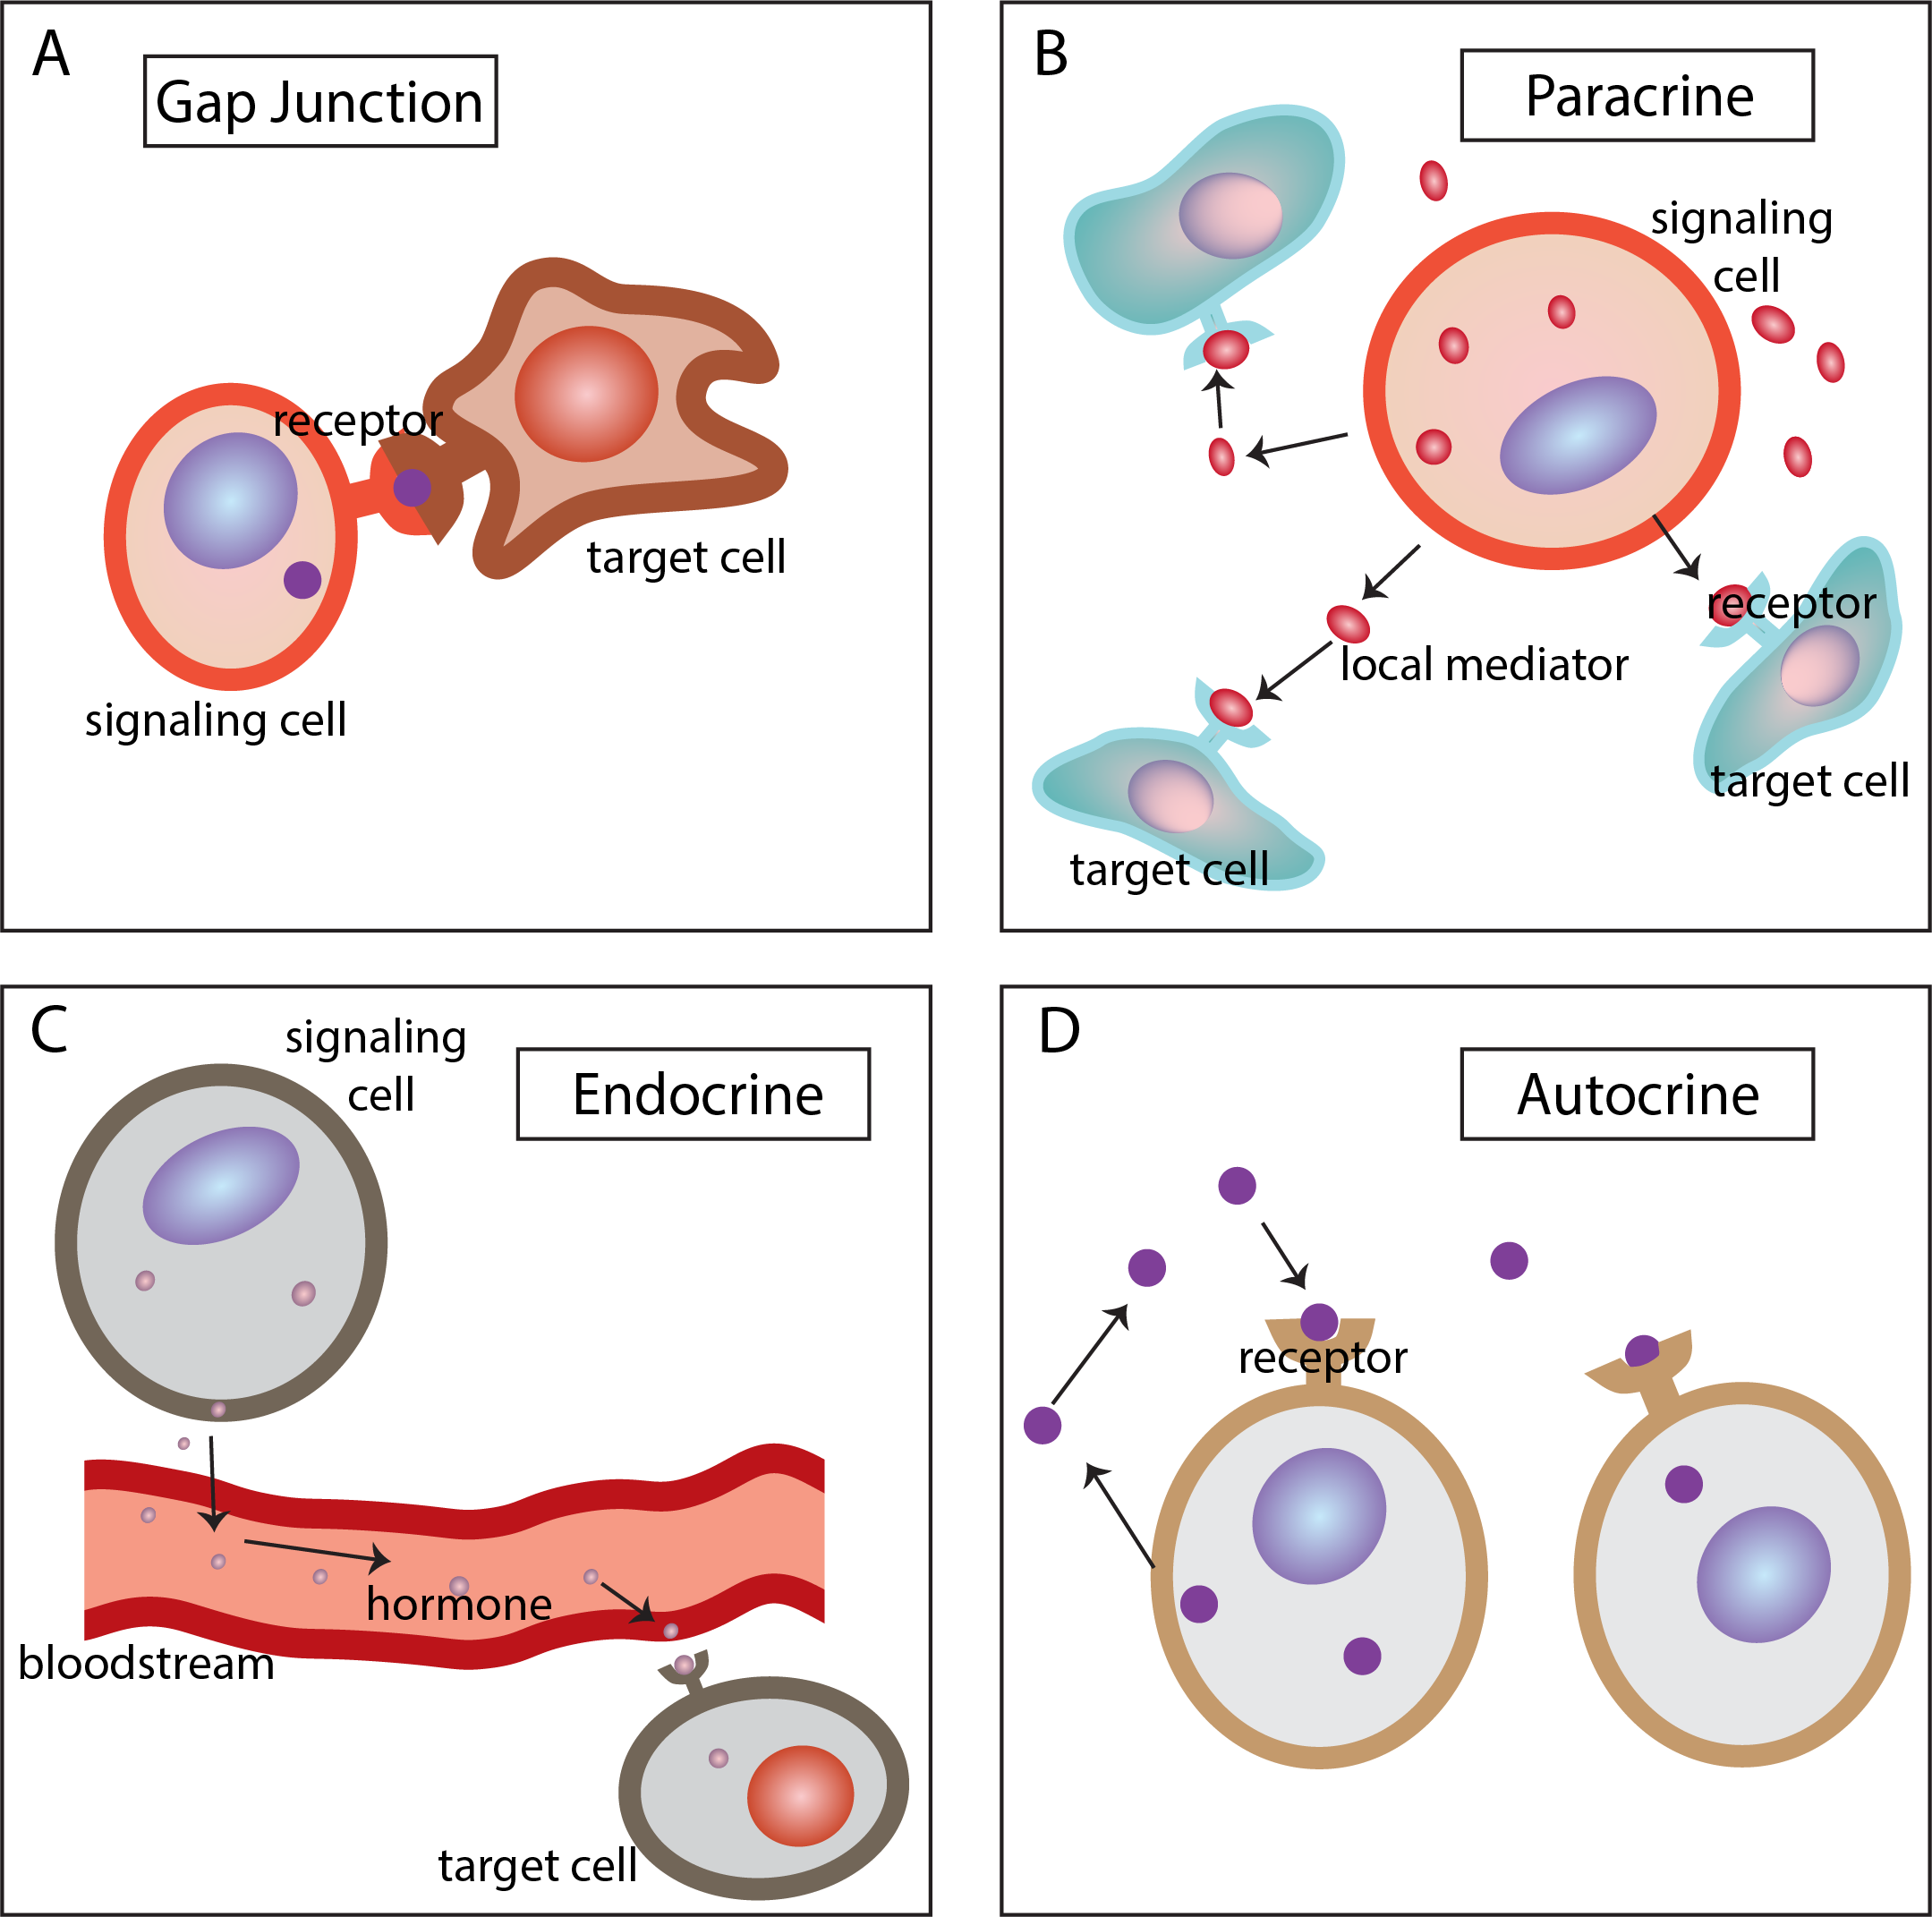
\includegraphics[width=0.8\columnwidth]{Chapter1/Figures/Chap1_figure2.png}
    \caption[4 Type of cell-cell interactions]{4 Type of cell-cell interactions: (A) Gap junctions is contact-dependent signalling which requires cells to be in the membrane–membrane contact. (B) Paracrine signalling does not require membrane-membrane contact, rather depending on local mediating signalling molecules that are released into the extracellular space and act on neighbouring cells. (C) Endocrine signalling depends on endocrine cells, which secrete hormones into the bloodstream for distribution throughout the body. (D) Autocrine signalling refers to cells secreting signalling molecules to induce the changes in the same cells}
    \label{fig:Chap1_figure2}
\end{figure}

Some cells can secrete signalling molecules to self-regulate or control other neighbouring cells of the same type. This type of communication is called \textit{autocrine signalling}. In \textit{autocrine signalling} (or intracrine signalling), cells stimulate themselves by sending the signalling molecules back to their own receptors. Autocrine signalling is most effective when occurring within the same cell or with neighbouring cells of the same type (Figure \ref{fig:Chap1_figure2}D). The process is used to encourage groups of cells to make the same developmental decision. Thus, autocrine signalling is often found in cells that are differentiated along a particular pathway to reinforce developmental decisions \cite{alberts2018molecular}. Autocrine signalling is also often found in cancer cells and enhances cell differentiation and proliferation \cite{sporn1985autocrine}.  

Every kind of cell, from the bacterium to sophisticated eukaryotic cells, can secrete chemical signals to perform cellular communication. The mechanism of cell signalling in single-cellular organisms such as yeast and bacteria has been well studied and understood \cite{alberts2018molecular}. Meanwhile, during the evolution of multicellular organisms, the signalling among cells achieved a high level of complexity. The crosstalks between different cell types from multiple tissues are crucial to every organism and form a complex microenvironment system to govern tissue functions. This is not only because the signalling methods are complex, but it is also because the number of cells present in the microenvironment can drive interaction to different outcomes. It is much more difficult to study the microenvironment system as a whole without a quantitative analysis and computational methods. Therefore, this thesis will hereinafter discuss only cell signalling in multicellular organisms, especially in humans and demonstrate the robustness of quantitative approaches to uncover the cellular communication system. 

\subsection{The biology process of cancer}
In all multicellular organisms, each individual cell is a part of the whole community and follows behaves in a socially responsible manner. To maintain the balance of the harmony of society, the number of cells in an adult body remains constant (around $10^{14}$ cells in an adult). However, throughout the lifespan, a cell can acquire some mutations which allow it to keep growing and dividing more than its neighbouring cells \cite{alberts2018molecular, greaves2012clonal}. Most of the mutated cells will be detected and either repaired or eliminated by the immune surveillance system in the body. However, cancer cells are said to be genetically unstable cells that accumulate enough mutations which give them \textbf{malignant} properties to break immunosurveillance and invade surrounding tissue. 

There are two malignant properties a cell needs to possess to be classified as a cancer cell. The cell needs to develop the mutations that allow it to (1) reproduce at abnormally speed, and (2) be able to invade and colonize tissue sites normally reserved for other cells. An abnormal cell that either increases in size or proliferates out of control will give rise to a neoplasm \cite{alberts2018molecular, hanahan2000hallmarks}. The combination of the two properties contributes to the fatality of cancers. As long as the neoplastic cells have not yet become invasive, the tumour is considered as \textit{benign}. A tumour is considered as \textit{malignant} when its cells have developed the ability to invade neighbouring tissue. Metastability is a dangerous characteristic of cancer cells. It even allows cancer cells to migrate to another part of the body through the bloodstream or lymphatic vessels and form secondary tumours \cite{alberts2018molecular}. The further a cancer cell metastasises the more resistant to eradication it becomes.   

The abnormal reproduction of cells fosters tumour progression and tumorigenesis. Most normal cells in the body have built-in safety mechanisms which limit the number of successive cell growth-and-division cycles (Figure \ref{fig:Chap1_figure3}) \cite{hanahan2000hallmarks, hanahan2011hallmarksnext}. These safety mechanisms consist of two distinct barriers: \textit{senescence}, a typically irreversible entrance into a non-proliferative but viable state; and apoptosis, which involves cell death (Figure \ref{fig:Chap1_figure3}A). Cancer cells are found to contain mutations that can disable normal safety mechanisms which is either an increase in cell division or an inhibition of apoptosis. In addition to the capability to alter built-in cell senescence and/or cell apoptosis, cancer cells are also resistant to cell stress and DNA damage. The tumour grows because the cell birth rate outweighs the cell death rate, but often by only a small margin (Figure \ref{fig:Chap1_figure3}B-C). Therefore, the time that a tumour takes to double in size is only a gradual process.

\begin{figure}[htp]
% \renewcommand{\figurename}{Supplementary Figure}
    \centering
    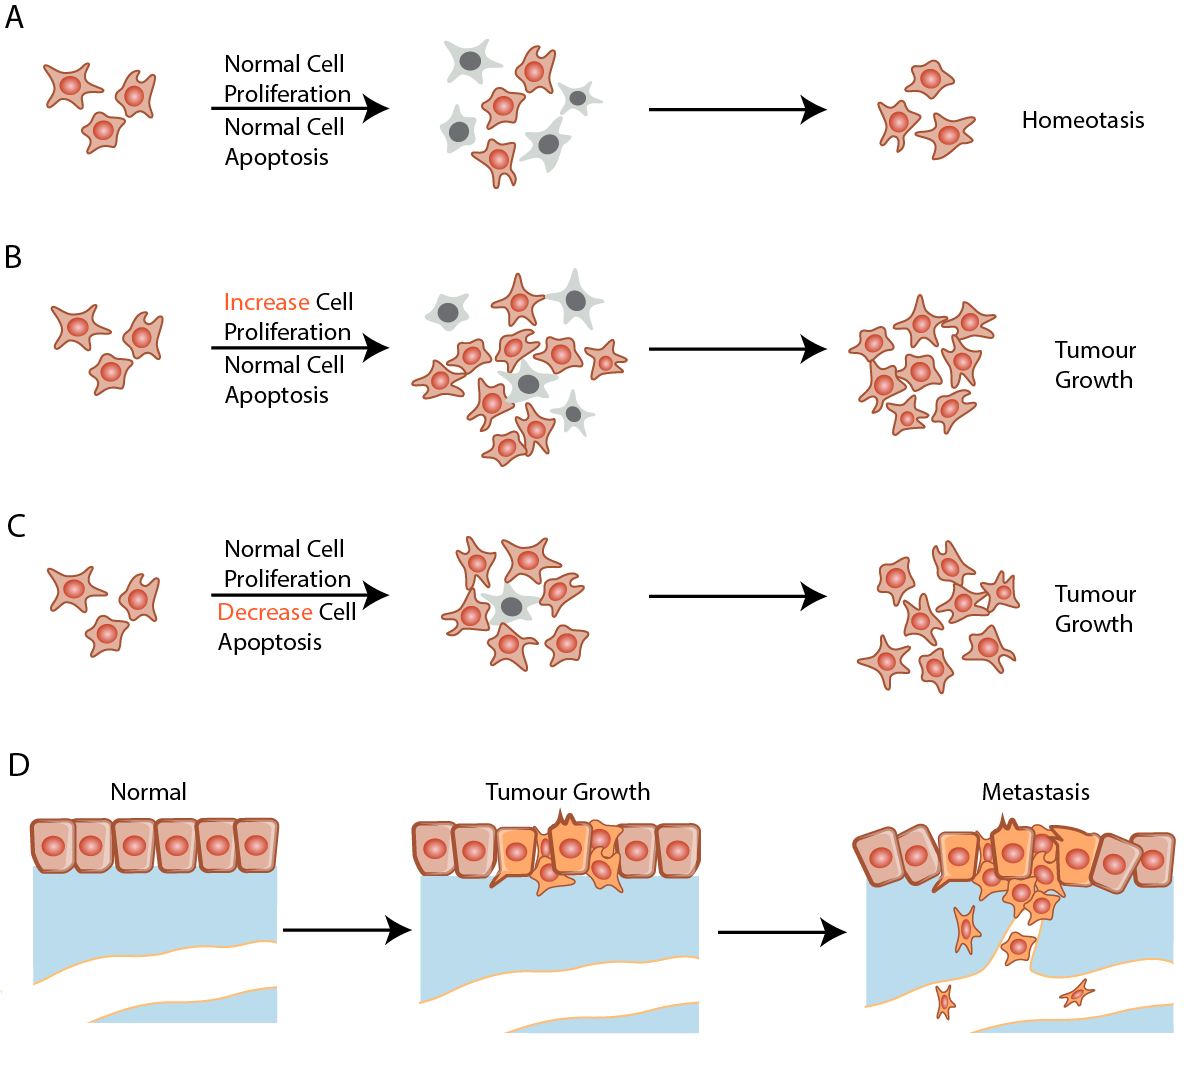
\includegraphics[width=0.7\columnwidth]{Chapter1/Figures/Chap1_figure3.png}
    \caption[Tumorigenesis and metastasis process. ]{The development of a tumour is the result of the mutated cells acquiring either stronger cell proliferation or inhibition of apoptosis (A-C). (D) An illustration of tumour cells resides from an organ to other organs through the bloodstream (figure adapted from \cite{alberts2018molecular})}
    \label{fig:Chap1_figure3}
\end{figure}

Metastasis is, in fact, a multistep process where cancer cells first invade locally, migrate to the circulation (lymphatics or bloodstream), and finally establish the new tumour at a distant organ. A cancer cell is dangerous due to its invasiveness and the ability to break free of constraints that keep normal cells in their designated organ \cite{greaves2012clonal}. Such properties are often acquired by the disorganized pattern of tumour growth and ragged borders, invading the neighbouring tissue. Fewer than one in a thousand malignant tumour cells that enter the bloodstream will colonise in a new organ and grow to the detectable secondary tumours \cite{joyce2009microenvironmental}. With modern blood test techniques, cancer cells can be detected early according to their surface properties while circulating in samples of blood from cancer patients. These biomarkers can inform the early treatment (\ie TP53, APC in colorectal cancer \cite{markowitz2009molecular}). 

While cancer cells tend to avoid apoptosis, this does not mean that they are immortal. In the interior of a large solid tumour, cell death often occurs on a massive scale. However, cancer cells within the tumour often die from necrosis process, which is unregulated death as the result of environmental perturbations. In necrosis, the cells become bloated and explode, releasing their contents into the local tissue microenvironment \cite{hanahan2011hallmarksnext}. Tumour necrosis factor (TNF$\alpha$) induces the upregulation of S100A8 and S100A9 in myeloid cells, which can increase metastasis \cite{hiratsuka2008s100a8, hiratsuka2006tumour}. 

The dynamic of genetic mutations within cells is the major cause of tumour initiation. However, it is generally agreed that cancer metastasis is partially constrained by a complex, multifactorial interplay between cancer cells and the host tissue microenvironment. Some microenvironmental features can promote neoplastic cells including infiltrating macrophages and neovascularization. Mathematical modelling is an ideal approach to dissecting mechanisms of cancer invasion as it can simultaneously and quantitatively consider interactions between multiple factors \cite{anderson2006tumor}. The following sections will discuss deeper about a different type of interaction within cancer and aim to address the need for a computational approach.       

\subsection{The role of cell-cell interaction within cancer microenvironment}
Tumour growth and cancer invasion are landmark events with location-dependent \cite{friedl2011cancer}. It is often known that cancer originates from genetic instability. However, the growth of cancer cells into the tumour and the process of cancer metastasis are constrained by cellular interaction and tissue spatial conditions that dictate the interaction within and surround the cancer nest \cite{west2019cellular, liotta2001microenvironment,anderson2006tumor}. Cancer cells can produce growth factor ligands themselves, to which they can respond via the expression of cognate receptors resulting in autocrine proliferative stimulation. Many epithelium cells in breast cancer can produce its family of epidermal growth factor (EGF) ligands to stimulate cancer cells proliferation and motility, suggesting they may participate in autocrine and signalling with cells of the tumour microenvironment \cite{nickerson2013autocrine}.  

Cancer clone habitats are not closed systems \cite{greaves2012clonal}. A unique ability of cancer cells is their quick mutation to different environmental conditions, affecting cellular morphology in order to survive \cite{clark2015modes}. Tumours consist of not only cancer cells but also a whole microenvironment including endothelial cells, smooth muscle, fibroblasts and inflammatory white blood cells. Cancer cells in a tumour are the group of cells that have accumulated dangerous mutations; however, the development of a tumour indeed relies on two-way communication between the tumour cells and the surrounding environment (tumour stroma). In cancer pathology studies, tumour microenvironment can influence cancer development in different ways. During early tumour development, the protection of the microenvironment surrounding the tumour fosters the tumour growth conditions such as chronic inflammation. As the cancer progresses, the cancer cells secrete signal proteins such as TGF-$\beta$ and EGF to stimulate normal cells within the tumour to induce epithelial development as well as to modify the extracellular matrix \cite{beck2011systematic,BREMNES2011209}. The stroma, in turn, secretes signal proteins that stimulate cancer cells' growth and division (i.e. CXCL12) \cite{kumar2018analysis,wang2017role}. There is a feedback loop of cell-cell interaction between the cancer cell metastasis and the tissue microenvironments; in which the increase in intratumoral cell-cell interaction promotes collective migration in cancer \cite{friedl2011cancer, whiteside2008tumor}, leading to dynamically induced disorganization of nearby microenvironments of the tissue \cite{friedl2012classifying, canel2013cadherin, almendro2013cellular, roussos2011chemotaxis, zervantonakis2012three}. The prediction of tumour stroma and cancer cell crosstalks has created a therapeutic strategy that aims to block cancer cell interactions with the environments to create the growth-fostering habitat called "ecological therapy" \cite{pienta2008ecological, calabrese2007perivascular, bissell2011don}. Knowledge of heterogeneity within the tumour and stromal compartments remains essential to understand the cancer development and evaluation of treatment progress \cite{pages2010immune}.

In addition to the interaction between cancer and the stromal cells, crosstalk between cancer and immune cells is also closely connected to the tumourigenesis process including progression and metastasis \cite{wang2017role}. The role of the immune system is to protect the host from infectious pathogens and remove damaged cells \cite{davis2007molecular}. Macrophages have been determined to play roles in both tumour elimination and increase of tumour malignancy \cite{wyckoff2007direct, chung2005molecular}. In the early stage of cancer progression, immune cells such as macrophages and myeloid secrete paracrine signalling molecules (i.e. CFS-1 ligand)  to trigger a cell death process to eliminate cancer cells \cite{wyckoff2007direct}. If cancer cells are completely cleared during this elimination stage, immune cells will remain around the cancer cells to suppress tumour growth \cite{bronkhorst2011detection, ly2010aged}. Studies showed that the presence of tumour-infiltrating CD8+ T cells and Th1 cytokines surrounding the tumours associates with favourable prognosis in different tumour types including melanoma, breast, ovarian, and colorectal cancer \cite{fridman2012immune, shalapour2015immunity}. At a later cancer stage, metastasis happens when the cancer cells can mutate and acquire a phenotype that helps them to elude immune system surveillance. For example, the increase of PD-L1 expression in epithelial cancer cells causes CD8+ T cell exhaustion, which subsequently promotes metastasis \cite{chen2014metastasis, wei2019combination}. In other words, the continuous cross signalling between immune-cancer cells exerts selective pressure on the cancer cells to become more motile \cite{giampieri2009localized,ilina2009mechanisms}. The growth of the tumour can be categorised as the consequence of cross-cell type communication and morphological dependence. As a result, the modelling of immune-cancer cell interactions creates great opportunities for tumour management through the development of targeted therapy including immunotherapy. Understanding the signalling molecules that are used by tumour-associated immune cells in the different stages of cancer progression will provide insights into current development immunotherapies.  

% ***************************************************
\section{Literature review}
\label{section:lit_review}
The wide application of single-cell sequencing technology has successfully identified rare cellular properties, molecular features of cell populations, and cell-cell heterogeneity in cancer research. However, cancer tumours comprise multiple layers of signalling across cell types which are location-dependent, making them more heterogeneous than expected. Gene expressions in a cell are dictated not only by molecular profiles but also by space (i.e. its position in tissues and/or organs) and time (i.e. stage of cell cycle or developmental stage of the organ) \cite{salomon2020genomic}. Therefore, the ability to integrate single-cell molecular profiles with the spatial context in studying cell-cell communication can benefit research about the potential treatment of cancer.

In this section, I will review the current development of experimental techniques and computational approaches to study cell-cell interaction through spatial transcriptomics and proteomics. The advances in experimental technologies have quickly evolved in recent years (Figure \ref{fig:Chap1_figure5}). Together with new technologies to spatially profile transcripts and protein expression introduced in the past decade, numerous computational methods have been developed. While some analysis packages or pipelines were developed alongside the experimental platforms, most of the complex cell-cell interaction models were designed to be universal across experimental designs. The section \ref{Chap1:Sub_Spatial_Experiment_Platform} will thoroughly review the key technologies in spatial transcriptomic and spatial proteomic. In particular Visium, RNAscope, Nanostring CosMx for spatial transcriptomic and Polaris, Imaging Mass Cytometry for spatial proteomics. Next, I will review the studies of cell-cell interaction methods which consider either non-spatial or  spatial context in section \ref{Chap1:Sub_Computational}.                

\subsection{Experimental approaches to cell-cell interaction}
\label{Chap1:Sub_Spatial_Experiment_Platform}
In the past, intercellular communication was examined by measuring intercellular electrical signals in the cell membrane \cite{bennett1966physiology, loewenstein1967intercellular, de1982cell}. The presence of gap junctions allows cells to exchange a variety of ions and small molecules, thus they reflect the cell\'s electrical permeability properties \cite{penn1966ionic, bennett1966physiology,loewenstein1966permeability,loewenstein1974cellular}. By utilising such electrical properties of membrane junctions, cell-cell communication can be measured by injecting a cell with one of the microelectrodes and the adjacent cells (with presumed shared gap junction channels) with the other microelectrode. This method is readily applicable for tissue types with widespread cellular communication through gap junctions \cite{penn1966ionic}. It has been used to unveil differences between cancer and normal cells within liver tissues \cite{loewenstein1966intercellular, loewenstein1967intercellular}. However, the disadvantage of measuring electrical signals between cells is that they can be highly tissue-specific (i.e. liver, heart and lens tissues) \cite{gros1983comparative}. Additionally, the throughput of such an experiment is very low. Therefore, measuring cell surface electrical signals through gap junctions has become less popular in recent years. 

Recent advances in high-throughput microscopy, sequencing technologies and antibodies research have fuelled the development of two fields called \textit{spatially} transcriptomics and spatial proteomics. In fact, cell-cell interaction within tissue context is a multi-dimensional problem. The most intuitive way to capture cell-cell signalling is through the imaging approach. Either confocal or two-photon fluorescence microscopy can capture high-detail images of intracellular structures in a cell. While a specific review of these two types of microscopy is beyond the scope of this thesis, it is worth noting that they both use laser light to excite fluorophores, with the resulting fluorescence captured by detectors. A great feature of fluorescence imaging is the ability to monitor a number of specific probes simultaneously, thus allowing co-localization or multiparameter imaging of structures within cells or tissues \cite{periasamy2013methods}. There exist a number of fluorescently tagged protein biosensors, which can be used to track the movement of some ligand molecules in the studies of cellular and molecular interaction in healthy and diseased tissues \cite{gerdes2013cell}. Although a number of studies, in the early 2000s, have been done to model and quantify the activity of ligands and/or receptors \cite{awaji1998real, go1997quantitative, maamra1999studies, sneddon2003activation, bohme2009illuminating} using imaging data, they have limited scalability (Figure \ref{fig:Chap1_figure5}). The number of target ligands and/or receptors that can be measured per experiment is limited by the antibodies or RNA probes that can be used concurrently.    

Regarding spatial transcriptomics, it is a general term referring to capturing and quantifying gene expression while retaining information of the tissue context \cite{burgess2019spatial}. There are several categories of spatial transcriptomic technologies. Current experimental technologies for spatial transcriptomics can be grouped into 4 major groups: (1) tissue microdissection-based approach, (2) RNA in situ hybridisation-based (ISH) approach, (3) in situ sequencing (ISS) approach, (4) in situ capturing and ex situ sequencing \cite{williams2022introduction}. Tissue microdissection-based is a brute-force approach to using a laser beam to dissect regions of interest from the tissue. These regions then undergo the RNA extraction and sequencing process. Due to multiple challenges in oncology settings and time-consuming, there are very limited spatial-omic studies utilising laser microdissection-based approaches \cite{wu2022spatial, wu2016spatially, junker2014genome}. Therefore, the following sections will discuss the other three spatially resolved transcriptomics approaches.
\subsubsection{In situ hybridisation (ISH)-based}

\label{section:Imaging_sequecing_review}
An interesting analogy for detecting a specific DNA sequence on the chromosomes or in a cell is like looking for a needle in a haystack. The needle is the DNA sequence of interest and, the haystack represents all chromosomes. This search is made much easier if the investigator has a powerful "magnet"—in this case, a fluorescent copy of the DNA sequence of interest \cite{Connor2008natureEdu}. The first attempt to localize mRNA was conducted in 1969 and used radioactive labels and hybridization probes in the nuclei of frog eggs \cite{pardue1969molecular}. To this day, radioactive probes are still available and seem to be the most sensitive choice. However, the high cost of the experiment and potential hazards make radioactive approaches less favourable. Soon after the first experiment with radioisotopes, fluorescent labels made great strides in replacing radioactive probes because of their safety profile, stability, and ease of detection \cite{rudkin1977high, Connor2008natureEdu}. Since the first demonstration in 1994 (\cite{bassell1994single}), numerous RNA ISH methods based on the fluorescent ISH (FISH) approach have been developed, including single molecule FISH (smFISH), RNAscope, sequential FISH (seqFISH), multiplexed error-robust FISH (MERFISH), expansion-assisted iterative (EASI-FISH), and most recently DNA microscopy. 

Most of the currently developed technologies for RNA ISH are FISH-based and use fluorescently labelled probes that are hybridized to predefined RNA targets, to visualize the presence of transcripts. Probes are either directly or indirectly hybridized to the RNA molecules and subsequently visualized by microscopy. A benefit of RNA ISH is the ability to characterise the presence of RNA sequences within the tissue without cells dissociation. Although the basic principle of FISH remains unchanged, the sensitivity and multiplexing capabilities have advanced considerably. The first attempt to increase the sensitivity of FISH protocol was in 2012 with the release of smFISH (single molecule FISH) \cite{ji2012single}. By using a set of 5 short oligonucleotide probes (20-50 bp) to target multiple regions of a transcript, smFISH produces a higher and more robust signal. However, smFISH can only target a few genes at a time and inherits the limitation of spectral overlaps in standard microscopy technology.

There is an improved version of smFISH, called seqFISH, which allows capturing more transcripts at a time through serial rounds of hybridization, imaging and probe stripping \cite{asp2020spatially}. In seqFISH, the fluorescent probes are one-hot encoded and undergo a sequence of hybridisation. Each round of probe hybridization, imaging and probe stripping captures the presence of up to 24 different transcripts separately and enables the profiling of 10,000 genes \cite{moses2022museum,eng2019transcriptome}. However, an increased number of hybridization rounds is also associated with more expensive and time-consuming (approximately 10 hours to conduct one sequence of probe stripping). 

In an effort to side-step the extensive time of seqFISH, MERFISH was first developed in 2015 \cite{chen2015spatially} using probes with two flanking regions. After hybridizing to the RNAs, the fluorophores will bind to two flanking regions to facilitate the imaging process. For every round of RNA capturing, only fluorescent bits are removed while the encoding probes remain. Computational error-correction is performed after readout to account for imperfect signals in one round. Therefore, each round of hybridization in MERFISH is less time-consuming (around 20 min) than those in seqFISH \cite{moses2022museum}. Similar to seqFISH, MERFISH can also profile a maximum of 10,000 genes. Most of the FISH-based spatial technologies available use either seqFISH-based or MERFISH-based barcoding. 

While these methods have the advantage of multiplexed detection, the FISH technologies rely heavily on the fluorescent signal from the probes. To increase the sensitivity of FISH, signal amplification of either target nucleic sequences prior to ISH (e.g in situ PCR) or signal detection after the hybridization process \cite{qian2003recent} can be used to enhance the quality of the image scanning. The signal amplification creates a quantification problem for RNA ISH and limits the application of RNA ISH in clinical analysis \cite{levsky2003fluorescence,wang2012rnascope}. Other RNA ISH technologies that can perform independent signal amplification such as RNAscope and DNA microscopy. While DNA microscopy is an optic-free mapping of nucleotides and does not rely on the physical location of cells, it is still a very new technology and has only been applied to a small subset of transcripts \cite{asp2020spatially,weinstein2019dna}. RNAscope technology is the more sensitive option for FISH which allows signal amplification and background suppression by itself.

Specifically, RNAscope assay is designed with ``Z-like" probes where the lower region of the Z is (18-25 bp) complementary to the target RNA and the upper region (14 bp) forms the binding site for the fluorescently labelled probes. Two assay probes with ZZ pairs are designed to bind in a region spanning 1000 bases of target RNA, this allows the specific detection and signal amplification from each target RNA molecule \cite{solanki2020visualization}. As a result, the RNAscope assay is best used for RNA sequences longer than 300 nucleotides. For short RNA sequences, a variant of RNAscope called BaseScope is a more suitable option. By using probe-specific amplifiers and sequence labelling, this assay can visualize multiple target RNAs simultaneously. Originally, RNAscope could only capture four different types of transcripts per experiment due to a limited number of spectrally discernible fluorescent dyes \cite{wang2012rnascope}. However, the latest version released in 2019, the Hiplex RNAscope assay has increased the number of RNA targets to twelve. Low multiplex RNAscope has been combined with another spatial proteomic technology called Imaging Mass Cytometry to capture both transcripts and protein simultaneously \cite{schulz2018simultaneous}. In comparison with seqFISH and MERFISH, RNAscope assays demonstrate lower multiplexing capability. 

To enable a faster imaging process while considering three-dimensional (3D) relationships of cells in thick tissue, expansion-assisted iterative fluorescence ISH (EASI-FISH) was introduced \cite{wang2021easi, borm2022scalable}. Before the ISH process, the RNAs within a tissue are preserved in a covalent attachment to the hydrogel mesh that covered the tissue. Next, the tissue in gel is hybridized with several rounds of fluorescently labelled probes, followed by cytosolic DAPI staining and imaging under light sheet microscopy. The 3D image reconstruction is generated by registering multiple 2D images of DAPI images and the transcripts of fluorescent beads from different cycles via an affine transform. The transcripts in 3D space are assigned to a cell within a disc of radius from the nuclei. Recent commercial techniques for 3D FISH are developed under the Nanostring CosMx platform \cite{he2022high}.  

The probes used in the CoxMx platform consist of two components. The RNA target-binding domain of length 35-50 bp followed by 60-80 bp of a DNA readout domain (reporter-landing domain). The readout domain is separated into four sub-domains which can be hybridised with unique 10-20 bp reporter probes. Each reported probe can be encoded by four different fluorophores making 64 unique reporters can be hybridised to the reporter-landing domain. Using that customisation, the CosMx platform inherits the capability to probe fluorescent signals in Z-stacked and alleviates the panel of RNA from 30 in EASI-FISH to 980-plex. Image registration is used to process 3D channel images from multiple rounds of hybridisation. An image processing algorithm is developed to detect the transcript fluorescent signal from the crowded reporter-binding event and assign it to the closest nuclei (within a radius of 0.5 pixel). Interestingly, the probe-encoded detection for RNA can be utilised for protein detection by replacing the readout sequences with antibodies \cite{he2022high}.   

The advancement of RNA ISH methods has not only allowed us to integrate the cells' functions with spatial information but also has expanded our understanding of the structural organization of normal and pathological tissues. FISH methods are becoming more popular in basic research. However, the use of that technologies in clinical routine is quite limited to validation of highly expressed genes (e.g EBER1/2 in EBV-related diseases) \cite{gulley2001molecular}. Over 10 tumour microenvironments  and 100 pairs of ligand-receptor specific for breast cancers have been discovered using the first demonstration of CosMx platform \cite{he2022high}. However, only a few methods have extended far beyond the inventor's laboratories and undergone successful commercialisation, including RNAscope, MERFISH, and CosMx \cite{conrad2022single}. 

\subsubsection{In situ sequencing (ISS) technologies}
An alternative to FISH is adapting signal amplification and in situ sequencing (ISS) of transcripts directly in the tissue. The concept of ISS methods is fairly similar to FISH when a panel of known sequence transcript is captured through the probes. The probes which have the padlock shape is a single-stranded DNA molecule containing the complementary sequence to the target transcript. Two ends of the padlock probes are closed by ligation, or by a DNA polymerase to create a rolling circle \cite{conrad2022single}. Sequencing by ligation is then used to read the actual RNA sequence of the transcript from padlock probes. The advantage of ISS approach over regular scRNA sequencing techniques is the capability to link the sequencing back to the location of the probes. The number of genes that can be profiled by ISS is limited by the barcode length \cite{williams2022introduction, asp2020spatially}. Just like in seqFISH, only a small subset of all possible barcodes given a barcode length is used for error correction.

The first example of this approach for spatial transcriptomics was released in 2013, when it was used to profile the gene expression in breast cancer tissue. The padlock probe binds to the cDNA through hybrisation and produced the  clonally amplified rolling circle of the target cDNA sequences. The rolling-circle product is sequenced by ligation for RNA and sequence tag. Imaging for each round of probe ligation is carried out to capture the signal of the rolling-circle products located in the tissue sample. Similar to seqFISH, the sequential steps of probe ligation, imaging, and washing are iteratively carried out until the number of bases has been identified. Before being acquired by 10X Genomics, the original ISS platform can profile 31 targeted transcripts used in breast cancer prognostic expression panel \cite{ke2013situ}. The recent release of Xenium can now profile up to 400 genes concurrently. 

To achieve higher throughput of RNA transcripts, fluorescence in situ sequencing (FISSEQ) combines the idea of fluorescently detection from FISH and cDNA amplification from ISS \cite{lee2015fluorescent}. First, a sequencing primer is hybridised to multiple copies of the RNA. Then, each RNA is in situ amplified via rolling-circle amplification. The fluorescent probes are introduced to separate the difference between cDNA strands. After several rounds of hybridisation and imaging, the fluorescent tags are stripped off and the sequencing is performed. By using the sequential approach in seqFISH and MERFISH, FISSEQ has the potential to profile a few hundred to a thousand transcripts. However, FISSEQ has several disadvantages including low fluorescent sensitivity and a long imaging process.  

The ability to generate mRNA sequencing profiles with location is a powerful tool. With enough transcript detected, this approach could be used to characterise the tissue compartment in cancer tissue without prior information  \cite{ke2013situ}. Although ISS has the ability to detect SNVs that would be missed in FISH, the sensitivity of this approach was much lower compared to some regular FISH approaches. Besides, several problems regarding the sequencing process of ISS have been identified. While the sequencing dropout rate in regular scRNA-seq is $10\%$, most ISS approaches have a dropout rate over $70\%$. The loss of detection events may be due to many factors, such as the loss of the
mRNA from the tissue due to long fixation degradation and target sequence dependency. Both ISH and ISS suffer some similar technical limitations, in particular a requirement for many hours to days of imaging time on a microscope, thus generating terabytes of data. Finally, these methods require some trade-off between capture efficiency and for a number of genes profiled. 

\subsubsection{Spatial barcoding and ex situ sequencing}
Another concept currently emerges as a promising technology for spatial transcriptomic which is to spatially profile the complete transcriptome by capturing and barcoding the transcripts \textit{in situ} followed by \textit{ex situ} sequencing \cite{asp2020spatially}. Many experimental methods have implemented spatially resolved transcriptomics through this concept. Since the first one called Spatial Transcriptomic (ST) was established in 2016, there have been a series of new technologies introduced including Visum, GeoMx Digital Spatial Profiler (DSP) and SpaTial Enhanced REsolution Omics-Sequencing (STEREO-seq). 

RNA capture efficiency can greatly affect the quality of these methods, especially at higher resolution. Since most of the current existing technologies for \textit{ex situ} spatial transcriptomics sequencing (ST—seq) are new, they often require tissue-specific optimization. The standard capture resolution currently ranges from 2$\mu m$ — 100 $\mu m$ which means the capture rate is close to fewer than 40 cells. However, the experimental costs are considerably lower than for ISS. Due to the capability to profile the full transcriptome, this approach is gaining more popularity.          

Among the technologies to perform ST-seq. ST was acquired by the company 10X Genomic in 2018 who is now providing commercial kits. The first version of ST—seq published in 2016 used surface glass slides printed with barcoded probes grouped into circle spots. Each spot has a specific barcode id that is unique to the x and y location on the glass slide. The tissue is fixed, imaged, and permeabilized on top of the spots. During the permeabilization process, mRNAs defuse out of the tissue and are captured by the probes. The final step is to reverse transcribe the mRNA and extract the barcoded cDNA-mRNA to sequence \cite{staahl2016visualization, berglund2018spatial}. With the latest release of the Visium Spatial Transcriptomic protocol (10X Genomics), with the advances in 3D printing, the diameter of barcoded spots is reduced from  100$\mu$m to 55 $\mu$m with a smaller distance between the spots.  Both  Visium  and ST have already been used for the analysis of the tissue heterogeneity and gene expression in tumour tissues \cite{berglund2018spatial, thrane2018spatially, moncada2019integrating,ji2020multimodal, yoosuf2020identification} and inflammatory tissues \cite{carlberg2019exploring}. Results from the studies applied to tumour tissues once again confirmed the role of the microenvironment in promoting tumour progression \cite{thrane2018spatially, moncada2019integrating}. Additionally, corresponding histopathology images of tissues stained with haematoxylin and eosin (H\&E) coupled with ST-seq allow the application of deep learning approaches for integrative analysis of histology images with the ST-seq profile \cite{he2020integrating, tan2019spacell}. Currently, protocols to enable recovery of mRNA from FFPE tissue sections for legacy ST or Visium are being extensively developed to facilitate higher sequencing depth.           

Besides Visium, STEREO-seq from BGI is another platform that captures the RNAs using an array of nanoballs printed on the chip. The standard nanoball in the chips has a size of approximately 2.2 $\mu$m diameter which is substantially smaller than the diameter of the spot in the Visium array. While tissue permeabilisation and RNA sequencing also follow the same principle of the other ST-seq approach, STEREO-seq outperforms Visum and legacy ST-seq with the ability to measure tissues at subcellular resolution.    

Given the complexity and heterogeneity of tumours, untargeted methods like Visium and STEREO-seq can extend the capacity to study immune cell infiltration both in localized and metastatic diseases. In comparison to RNA ISH or ISS, ST-seq provides sub-optimal spatial resolution. However, with the advantage of the whole transcriptome profile, ST—seq is undoubtedly a promising complementary technology to FISH and/or ISS.  
% \subsubsection{Barcoded-targeted sequencing and }
% \subsubsection{Spatially barcoded probes and ex situ sequencing}
% These techniques are generally transcriptome wide, but do not have single cell resolution; the resolution is the size and shape of the spots and spacing between the spots. In ST and Visium, the array is constructed by printing the capture sequences onto commercial microarray slides, so the 5’ end of the sequences are attached to the slide; where each spatial barcode is placed is known. 

\subsubsection{Fluorescent-based spatial proteomic technologies}
Similar to spatially resolved transcriptomics, spatial proteomics often refers to the set of methods that use imaging technology to capture the presence of proteins in their native cellular environment without the need for the physical separation of cells or organelles before proteomic analysis. In addition to understanding the morphological context of RNAs, the spatial distribution of proteins is also equally important in studying cancer. Protein localization directly connects to protein function in health and disease. Being able to capture the localization of proteins and their dynamics at the cellular level is essential for a complete understanding of cell biology \cite{lundberg2019spatial}. 

There are several technologies to visualise the presence of proteins within the spatial context. These approaches are often grouped on either highly multiplexed imaging or mass cytometry imaging technologies. Similar to FISH technologies, multiplexed imaging is a fluorescence-based/colour-based approach and involves iterative rounds of staining, imaging, and removal of signals. Immunofluorescence (IF) and immunohistochemistry (IHC) are technologies used for visualizing cellular components, especially proteins which are categorised into the multiplexed imaging approach. They were invented in 1904s by Albert Coons \cite{coons1941immunological} and remain a cornerstone in pathology and health care. Since the development of IHC and IF, the number of studies that used these techniques has grown exponentially. These methods are commonly applied by the cellular biology, biochemistry, pathology and immunology fields and reflect the particular value of IHC and IF in researching diseases.        

IHC is a general term for the techniques that use antibodies or enzymes to identify specific proteins (antigen markers) in cells within tissue sections. The antibodies are specific and are expected to only bind to the targeted proteins. There are many different ways to perform visualization of targets in tissues with IHC or IHC-based methods. However, based on the experimental settings, IHC can be categorized into two groups: colourimetric and fluorescent. In colourimetric IHC, the antibodies or enzymes bind to proteins and trigger coloured precipitation which becomes visible to standard light microscopy \cite{BOURGEOIS2014132}. The enzymatic reaction or coloured precipitation keeps producing products as long as there is no more regent or physical space to deposit more reactant \cite{corthell2014basic}. Consequently, the colourimetric staining IHC is permanent in the tissue section and can be used for qualitative analyses where quantification is not considered important \cite{seidal2001interpretation}. 

Visualization of antigens by fluorophore-conjugated antibodies is also often referred to as IF \cite{joshi2017immunofluorescence}. Unlike colourimetric IHC, fluorescence IF is not stable over long times and can only be observed after excitation with specific wavelengths \cite{corthell2014basic}. The antibody, when excited emits light of a different wavelength. IF also inspired the use of fluorophore-conjugated probes to directly visualize specific DNA and RNA sequences in the tissue which is often referred to as fluorescent in situ hybridization (FISH). There are two different fluorescence assays available for detecting antigens which are categorized by whether a single antibody or two antibodies are used, namely direct and indirect IF \cite{JOSHI2017135}. The former protocol is simpler and used for labelling abundant target proteins with a primary protein carrying a fluorophore that binds to a specific antigen. Meanwhile, the indirect IF protocol requires multiple stages of incubation; a primary antibody that binds only to the target and a secondary antibody with fluorophores to attach to the primary antibody. The primary antibody in indirect IF can allow multiple secondary antibodies to bind to it, creating signal amplification effects. Therefore, indirect IF is a better choice for detecting low-abundance targets. In comparison to colourimetric IHC, the benefit of using fluorophores is that they label multiple targeted proteins in the same tissue sample. However, unlike colourimetric staining, fluorescent labelling is not permanent. Since the fluorescent signal generally reflects the concentration of bound antibody \cite{dabbs2017diagnostic}, IF is considered a better choice for a quantitative experiment.

Due to relatively low costs, IHC and IF have been playing a central role in the visualization and identification of tissue antigens as well as in clinical diagnosis and prognosis for years \cite{ducheyne2015comprehensive, rupprecht2015current}. Depending on the purpose of the experiments and tissue preservation technique, IHC or IF be used interchangeably. While IHC studies are routinely used for pathological clinical diagnosis, the IF technique is the method of choice when an experiment requires investigation of colocalization of multiple proteins \cite{joshi2017immunofluorescence}. IHC and IF can be done on fresh frozen tissue yet most IHC is performed with Formalin-Fixed Paraffin-Embedded (FFPE) tissue. An example of the application of immunostaining in a clinical context is the used of IHC to evaluate the presence of HER2 in breast cancer sections. By using IHC and antibodies to detect HER2 receptor, clinicians can diagnose the current status of the patient to better decide on treatment options. Clinically, immunostaining is used for histopathology for the diagnosis of specific types of cancers based on known molecular markers.  

% [Polaris]
The results of IHC and IF heavily rely on the antibodies of choice and the capabilities of the technician performing them. Many studies highlighted that the choice of the antibody panel and the interpretation of the reaction patterns are the most important factors for  clinical outcome \cite{de2010immunohistochemistry, jensen1997immunohistochemistry}. In laboratory science, immunostaining by IHC and IF is limited by the number of protein markers it can feature at one time. Thus, IHC and IF are still being optimised for better performance in a multiplexed manner \cite{joshi2017immunofluorescence}. It is worth noting that protein visualization using fluorescence-based staining remains a good option. Polaris, as an example, provides a multiplex IHC based on the OPAL technology that can capture up to 9 proteins with very high quality. High-throughput multispectral scanning from Polaris can produce a whole slide scan of 6 biomarkers in 6 minutes ($1x1.5cm$ tissue section) \ref{hoyt2021multiplex,marc201934th}. The increase in signal accuracy can reduce the false colocalisation and signal crosstalk between biomarkers. The average signal intensity for all the markers has been validated to be within the recommended range ($10-30$) \ref{donovan2021924}.  
% []

There are multiple technologies for multiplexing fluorescence-based protein staining including NanoString GeoMx and co-detection by indexing (CODEX). In Nanostring GeoMx, a multiplexed cocktail of primary antibodies with  unique ultraviolet-photocleavable DNA oligos is used to target the proteins. After exposure to ultraviolet light from the GeoMX instrument, pools of released indexing oligos were hybridized to the optical barcodes and then read by another instrument (e.g NanoString nCounter or Illumina MiSeq) \cite{de2020unraveling, helmink2020b}. This enables to simultaneous detect up to 96 proteins and over 1000 RNA targets. CODEX has been developed by the inventor of MIBI and also uses a specialized instrument to convert images from fluorescence microscopes into highly-multiplexed imaging systems. CODEX currently allows the detection of over 60 protein markers within the tissue by iteratively staining and scanning the tissue sections\cite{goltsev2018deep}. A disadvantage of CODEX, but also of many other FISH-based technologies and IMC, is the lack of signal amplification which results in the under-detection of lowly abundant protein/gene markers. A comparative overview of three different approaches to performing spatial proteomic is shown in Table \ref{table:SpatialProteomicComparison}. 

\subsubsection{Mass Cytometry Imaging Technologies}
In addition to more recent advances in IHC and IF, there are now several new protein imaging technologies based on mass spectrometry that allow the multiplexing of numerous proteins (up to 100 protein markers) with huge potential applications in research, especially for cell colocalization and interaction studies within tissues. Recent developments in flow cytometry, high-throughput microscopy and mass spectrometer have enabled to apply conventional protein study strategies in a spatially resolved context. The first wave of spatial proteomics methods used mass cytometric (MC) analysis. As an off-shoot from IHC/IF technology, MC-based spatial proteomic methods use antibodies to visualize the protein. An advantage of this type of analysis approach is that it can easily be used to study proteins in many different cell types. Two notable technologies have been developed that are based on the MC approach including Hyperion Imaging Mass Cytometry (IMC) as the pioneer and Multiplex Ion Beam Imaging (MIBI) as the direct competitor platform. Both methods use antibodies conjugated to stable metal isotopes. In IMC, after the tissue section is immobilized on slides, the tissue is stained with panels of antibodies then it enters a laser ablation chamber where it is rasterized until it plumes. The aerosolized/ionized plumes of tissue are fed into a time-of-flight mass spectrometer for analysis of isotope abundance.  There was a study that combined two technology of RNAscope and IMC workflow to interrogate the interplay between transcription and protein in the tissues \cite{schulz2018simultaneous}. Instead of using fluorophores, the RNAscope probes are modified to tag with metal. Thus mRNA and protein can be simultaneously measured in single cells. By using pure and rare-earth element isotopes, IMC can overcome the limitations of spectral overlap observed in IF and allow quantifying up to 38 tagged channels simultaneously. However, the use of lasers damages the tissues that are being scanned.

Alternatively, MIBI can be used to image histological sections labelled with isotope-tagged antibodies. Most of the steps for measuring protein levels using MIBI are similar to IMC. However, in MIBI secondary ion mass spectrometry is needed and  an (oxygen) ion beam is used instead of laser ablation to raster over the tissue. Subsequently, ions are analysed using a mass spectrometer. While the MIBI only ablates a thin layer of the tissue (20-50nm) and cause fewer damages, the technology creates matrix effects and makes quantification more challenging \cite{bodenmiller2016multiplexed}.

There exists another branch of technology called Mass Spectrometry Imaging (MSI) that characterises protein expression using a mass spectrometer. Matrix‐Assisted Laser Desorption/Ionization (MALDI) tissue imaging is a technology using this approach and has been proven to be more versatile than MC. In MALDI, a laser and mass spectrometer are used to ablate the tissue and ionize the molecules. Eventually, the ionized molecules are fed to the spectrometer to determine the molecular weights \cite{caprioli1997molecular}.  This is performed in a label-free manner to measure the proteins present in the tissue. In this way, MALDI is more suitable for non-targeted experiments. However, there are also a number of limitations for MALDI or MSI in general such as lower spatial resolution, reduced sensitivity for larger proteins, and low multiplexing capability. 

\begin{table}[ht]
\centering
\caption{Feature comparison of spatial proteomic technologies}
\begin{tabular}{||P{3cm} || P{3.5cm} || P{2cm} || P{2cm} || P{2cm} ||} 
 \hline
   & Staining IF   & \multicolumn{3}{c||}{Mass tagged antibodies} \\  [0.33ex] 
 \hline\hline
 Technologies & CycIF, CODEX, NanoString DSP  & IMC & MIBI & MALDI   \\ 
 \hline
 Resolution & $\sim$600$\mu$m-single cell  &  $\sim$1000$\mu$m & $\sim$260$\mu$m & 50-200$\mu$m \\
  \hline
 Repeat analysis  & Yes  &  No & Yes & Yes \\
  \hline
Maximum epitopes  & $\sim$60-96 & $\sim$40 & 40 & $<$10   \\ [1ex] 
 \hline
\end{tabular}
\label{table:SpatialProteomicComparison}
\end{table}
\subsubsection{Challenges and general considerations}
While in some cases a single technique might be sufficient, more often the combination of single-cell multi-omics and imaging technologies is required to solve the complexity of cell communication in cancer (Fig.\ref{fig:multimodal_approach_cci}). The availability of mass spectrometry imaging and staining technologies might gradually replace the position of IHC and IF in laboratory research. However, until the new technologies are mature enough, clinicians still rely heavily on the use of IHC and IF. In addition, we need more advanced technologies which allow the acquisition of molecular profiles from single cells without the need of dissociating them from their tissue context  \cite{de2020unraveling}.

% \subsubsection{}
% \subsubsection{}
\subsection{Computational methods to study cell-cell interaction within spatial context}
\label{Chap1:Sub_Computational} 

As discussed above, an important feature of the cellular phenotype is its morphology. While scRNA-seq data can provide information about gene expression in cells, cell morphology is about cell physical features such as locations, area, perimeter, solidity, eccentricity and circularity. Additionally, both gene/protein expression and cell morphology are important features, especially in a disease context. The emergence of multiplexed spatial analysis enables dissecting the tumour microenvironment at multiple levels and higher granularity. 

\subsubsection{Cell-cell interaction inference using scRNA-seq based data}
To perform the computational study of cell-cell interaction, we need to address the two disadvantages of (1) a limited number of markers and (2) a lack of information on spatial location. The widespread use of single-cell data, over the past few years, in the form of single-cell RNA sequencing (scRNA-seq) has unveiled rare cellular functions and biologically meaningful cell-to-cell variability. Many computational methods have been proposed to infer the ligand-target links between cells  from scRNA-seq data such as CellPhoneDB \cite{efremova2020cellphonedb}, NicheNet \cite{browaeys2020nichenet}, SingleCellSignalR \cite{cabello2020singlecellsignalr}, NATMI \cite{hou2020predicting} and iTalk \cite{wang2019italk}. While scRNA-seq loses the spatial information, the method can measure a higher throughput of transcripts. Cell dissociation is required in order to perform scRNA-seq experiment. The dissociation procedure causes a loss of cell coordination information, making it challenging to link the transcriptomes back to their original spatial location. As discussed, the spatial context in cancer is a critical component for studying cell-cell interaction. Subsequently, these packages for cell-cell interaction inference from scRNA-seq data are used as biomarker discovery tools and required validation \cite{de2020unraveling}. 

To overcome the lack of spatial information from scRNA-seq prediction, a complementary approach that integrated multiple modalities with scRNA-seq data and spatially-resolved data has been used. Integrating spatial context into studying cell communication would greatly improve the justification of the ligand-receptor inference result and satisfy the grasp for modelling intratumour heterogeneity and cell communication during tumour development \cite{crosetto2015spatially, pages2010immune, marusyk2012intra,bedard2013tumour}. Recent studies combined scRNA-seq to spatial transcriptomic to locate the interaction within immunosuppressive tumour-specific keratinocyte subpopulations in non-melanoma skin cancer \cite{ji2020multimodal}. Such integrated data may offer insight into clinical prognosis. However, there is still a gap in computation when integrating spatial proteomic with scRNA-seq data. In many cases, a third experiment is required for a holistic integration \cite{ji2020multimodal, schulz2018simultaneous, govek2021single}.    

\subsubsection{Ligand-receptor interaction inference using spatially resolved -omic data}
Given the advances in spatial-omic experimental methods, we can now capture simultaneously up to 900 different transcripts and 40 proteins markers from a sample. It is natural to ask whether we can perform cell-cell interaction from spatial-omics data independent from scRNA-seq data. To address that,  several computational approaches have been developed to enable the data analysis of spatially-resolved multiplexed data. 

stLearn uses the curated CellPhoneDB database to make inferences about the L-R pairs that co-express by the cells from neighbouring spots. The p-value of the coexpression is computed by permutation test of the observing L-R pair aganst the null distribution. Then regions with diverse cell types (from Seurat label transferring or cell type deconvolution) and L-R coexpression in neighbouring spots are identified as regions where cells are likely to be signalling to each other. A similar strategy is used in Giotto. Giotto identifies cell type colocalization by labelling edges of the spatial neighbourhood graph as homo- or heterotypic and permutes cell type labels to find whether the cell types are more or less likely to colocalize than expected from completely random cell type localization. L-R coexpression in neighbouring cells on the spatial neighbourhood graph from two cell types is identified and the p-values of the coexpression scores are computed by permutation testing, permuting locations of cells within each cell type. Within one cell type, Giotto uses classical DE (Student’s t-test, Wilcoxon rank sum test, limma, and permutation of spatial locations) to find DE genes between neighbours of cells of another cell type and non-neighbours.

In GCNG (Yuan and Bar-Joseph 2019), the spatial neighbourhood graph is constructed as an edge that connects a cell to its 3 nearest neighbours. Then both the gene count matrix and the normalized Laplacian of the neighbourhood graph are fed into a graph convolutional neural network (GCN), which is trained on known L-R pairs. The GCN can then predict novel pairs of genes involved in signalling, and if trained on the direction of interaction in the L-R pairs, it can also predict the direction of causality in the novel pairs. With the cell-cell distance matrix, another optimal transport plan from ligands to receptors can be inferred, interpreted as how likely one cell communicates with another. A disadvantage of spatial neighbourhood graphs is that the common ways of construction are somewhat arbitrary. For instance, k nearest neighbour is a common way to construct the graph, but this k is somewhat arbitrary, although cell signalling can occur over a distance with secreted ligands.

\subsubsection{Cell types colocalisation analysis}
Several spatial analysis packages consider each cell as a point in a 2-dimensional coordinate system including squidpy, spicyR, etc. The advantage of this point-process approach is that it can use most of the analytical procedures established in high-level spatial analyses in social studies \cite{yushimito2012voronoi}. It is reasoned that the spatial structure of the tissue is a heterogeneous collection of single cells, consisting of multiple homogeneous groups \cite{schurch2020coordinated}. In this approach, we can identify spatial communities throughout the tissue using $K$ nearest neighbour and/or a radial distance approach (Fig: \ref{fig:CCC_conceptualised}A). For each cell across the tissue, the spatial identity of itself is defined by a K number of nearest neighbouring cells (including itself as the reference). The nearest neighbour metric is measured by the Euclidean distance between the $X$ and $Y$ coordinates of the cells in the two-dimensional tissue section. Alternatively, we can also apply a neighbourhood identification method that is threshold-free, known as the Delaunay cell network \cite{guibas1985primitives, dries2021giotto}. The spatial identities of cells are then clustered by their neighbourhood features \ref{fig:CCC_conceptualised}. The clusters of cells based on cell neighbourhood (i.e. spatial identity) can reveal communities of cells within the tissue and the composition of cell type for each community. Such methods have been used and adopted in different fields including eco-geography as well as biology \cite{goltsev2018CODEX, dries2021giotto}.

To ascertain whether cell communities identified by the above approaches followed true spatial patterns, co-occurrence analysis also employs similar principles as in the nearest neighbourhood approach. This co-occurrence analysis was inspired by an approach introduced by \cite{tosti2021single}, first applied for spatial transcriptomics data of human pancreas \cite{tosti2021single}. The co-occurrence score can be estimated by the Equation \ref{Eq:Cooc_equation}, which is defined by the fraction of the probability of observing a test cell type $exp$ at the presence of a reference cell type $cond$ ($P_{r}(exp|cond)$) over the probability of observing that test cell type $exp$ $P_{r}(exp)$ at the presence of any other cell type within the same distant interval $r$. At a specific distant $r$, $Co_{r}$ indicates how high/low $exp$ and $cond$ cell types co-localised compared to random cell types. The comparison of $Co_{r}$ at an increasing distant radius $r$ shows how the co-localisation of two cell types starts dispersing.


\begin{align}
\label{Eq:Cooc_equation}
Co_{r} = \frac{P_{r}(exp|cond)}{P_{r}(exp)} 
% K(t) =  \sum_{i=1}^{n}\sum_{n}^{j}1\{d_{ij} < r\} \\ 
\end{align}

Histocat's neighbourhood analysis uses  basic statistical methods to find significantly enriched interactions between or within cell type. The pairwise interactions of every cell are defined by the user (6 pixels) (Figure \ref{fig:CCC_conceptualised}B). Using the cell segmentation masks as the representation of the cells, a neighbour is defined as a pair of cells within the pixel distance selected during the loading process. The pairwise interaction was compared to a random distribution using two individual one-tail permutation tests within the same image. The test suggested how significant a pairwise interaction between two cell types was compared to random, and eventually suggested an interaction or an avoidance. The comparison to a matched randomized tissue for every individual image controls for both the distinct connectivity and the specific cell types in that tissue. 

\begin{equation}
\begin{split}
P_{lt} = \frac{ \sum(mean(permutation) \leq mean(real\_data) )}{number\_perm + 1} \\
P_{gt} = \frac{\sum(mean(permutation) \geq mean(real\_data) )}{number\_perm + 1}
\label{chap1:eq:02}
\end{split}
\end{equation}
Where $P_{gt}$ and $P_{lt}$ defined $P$ value for each tail, 
The absolute cell number or the size of the image does not have a direct effect on the neighbourhood analysis; only the frequencies of cell types present and the relative quantities are important. 
\begin{figure}
    \centering
    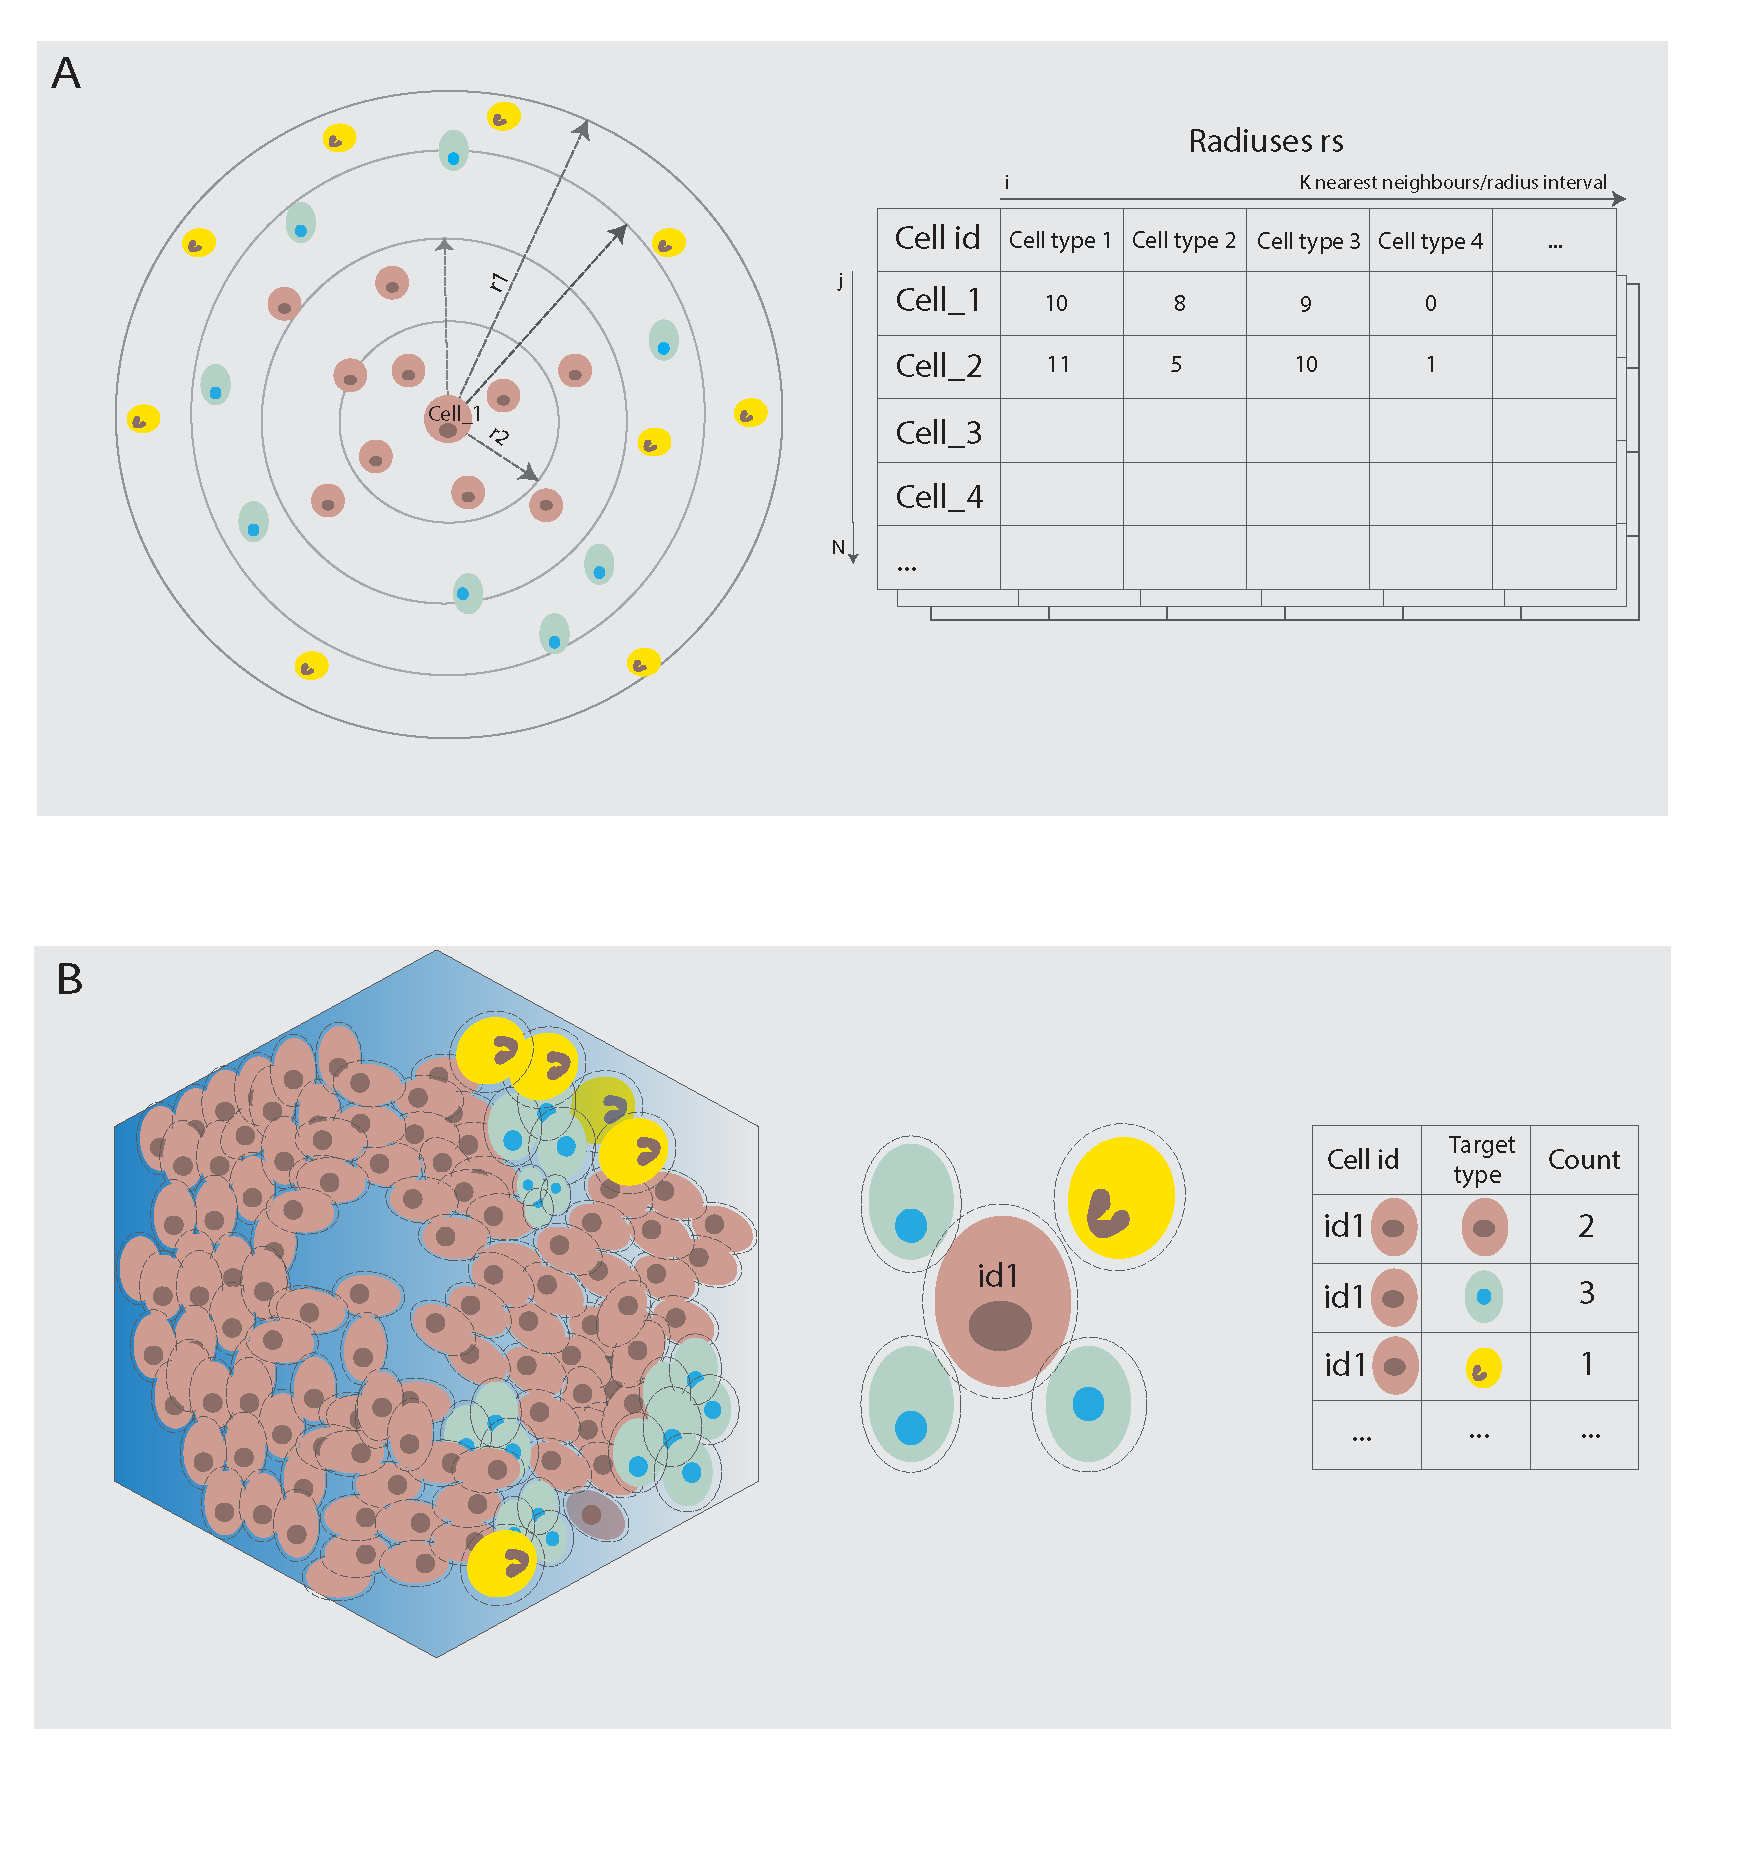
\includegraphics[width=0.85\columnwidth]{Chapter3/Figures/Conceptualise_CCC_analysis_cropped-01.png}
    \caption[Summary of different cell type interaction analyses.]{Summary of different cell type interaction analyses. (A) Schematic of cell-cell interaction through varied distance interval. The analysis process starts by iterating through every cell then accumulates the information about neighbouring cells to determine the cell spatial identity. (B) Schematic of measuring spatial interaction of cells through counting the number of touching cells. Randomising is applied at the downstream of the analysis to identify the significance of pairwise interaction}
    \label{fig:CCC_conceptualised}
\end{figure}
% squidpy is another analysis package that provides a thorough spatial analysis and visualisation of any given spatial -omic data. The squidpy packges is builts on   

% Spatial variance component analysis (SVCA) (Arnol et al. 2019) models the expression of each gene of interest among the cells as a 0 mean Gaussian process. The covariance h
% [...]
Despite the described experimental advances in imaging and sequencing technologies, there are limited computation approaches that have been developed to enable and expand the analysis of the data. Most open-source tools that provide image-linked data analysis workflows were typically developed for low-plex fluorescence microscopy (e.g IHC and IF) and were not geared to apply in analysing highly multiplexed measurements. Some emerging open-source software tools provide highly interactive graphic interfaces and are more user-friendly graphic such as QuPath, CellProfiler and HistoCat. These open-source software programs have the advantage of customising analysis modules which allow users to implement and optimise the analysis of their own. It is also worth noting that open-source software programs are widely popular among the research community. Thus, the user community and support are more available  than that of commercial software. 

Meanwhile, there is a number of analysis packages that do not provide a graphical interface but can control every function inside such as Spatial Seurat and scanpy. The advantage of having control of analysis through script is that they allow to scale up the amount of data easily. These packages are more suitable for bioinformaticians and those who have a computational background. However, they often abandon and undervalue spatial information while focusing more on sc-RNAseq profile. It necessary to interrelate and utilise layers of information obtained from spatially resolved omic data. There is still a lack of analysis software that can properly address the need to incorporate multiple types of data as well as provide the capability to scale up the analysis.


\label{subsec:ST_seq}


% \subsubsection{RNA in situ hybridization (ISH)}


% \subsubsection{Spatial proteomics}

\section{Research Objectives}
The rise of immunotherapy is substantially changing the cancer treatment paradigm \cite{dobosz2019intriguing}. However, less than $30\%$ patients respond to a single treatment type \cite{ott2017combination}. In addition, immunotherapy also associates with a variety of severe autoimmune-like side effects \cite{naidoo2015toxicities,bertrand2015immune}. These can be attributed to heterogeneity among single cells within the tissue. Technologically, single cell multimodal omics integration is recognized as the method of the year for 2019 by Nature Methods \cite{teichmann2020method}. By simultaneously measuring multiple modalities, we can gain insight of different aspects of one cell at a time. Thus, it can greatly inform the discovery of relationships across cell types and relationships across -omics \cite{teichmann2020method}. The expansion of spatial -omics data further improves our understanding of different angles of cell communication in cancer as well as the finding of rational immunotherapy agents. Since both discovery and translational research goals investigating cell communication rely on the integration of spatial-omics datasets, this thesis will be focused on adapting and developing analysis methods to combine imaging and sequencing data to investigate intercellular communication.   


% The overarching hypothesis of thesis is: \textbf{a large number of cell-cell interactions in cancer can be identified and characterised by spatial omic data.}. 
\section{Thesis Overview}
\subsection{Overview of the analysis methods named STRISH to study cell colocalisation in SCC/BCC skin cancer samples}

Chapter 2: Using Spatial Transcriptomic and single-cell RNA sequencing for cell-cell communication. 

Cell-to-cell communication underscores a dynamic cellular ecosystem that develops, evolves, and responds to environmental factors. The implications and roles of cell-to-cell communication have been investigated extensively, particularly in cancer, using a wide range of in vitro and in vivo techniques, albeit at different scales and resolutions \cite{brucher2014cell}. Breakthroughs arising from discoveries in cell communication have led to important clinical applications. 
% A classic example is the interaction via immune checkpoint proteins \cite{pardoll2012blockade}. Tumor cells, tumor infiltrating lymphocytes and tumor associated myeloid cells express inhibitory PD-L1/CTLA4 ligands to engage PD-1 receptors on cytotoxic T cells and CD80/86 receptors on myeloid cells, effectively blocking immune activation against the tumor cells. The discovery has led to applications of using monoclonal antibodies that specifically target this ligand-receptor (L-R) interaction as a form of immunotherapy, allowing immune cells to suppress cancer growth \cite{weiner2012antibody}. Therapies targeting these two pairs of ligand-receptors have transformed the management of several cancers, including melanoma, renal cell carcinoma, bladder cancer, head and neck cancer, and many others \cite{ott2017combination}. Notably, often less than 20\% of patients respond to a single immunotherapy, including common cancer types like breast, colon and prostate cancer \cite{ott2017combination}, and hence the urgent need to combine therapies, for example by using antibodies against PD-L1, CTLA-4 and/or PD-1 \cite{ott2017combination}. However, mechanisms of action for combinational immunotherapies remain elusive \cite{wei2019combination} and the number of current druggable targets for cancer-immune cell interaction is extremely limited, compared to the large repertoire of over 2,000 known ligands and receptors. Therefore, research to explore and advance understanding of known and new ligand-receptor pairs in the context of tumor-immune cell interaction within a tumor is extremely important for the further development of immunotherapies \cite{weiner2012antibody, helmy2013cancer}. 

Most ligand-receptor (L-R) interaction research so far has been relying on the use of fluorescently-conjugated antibody-based methods, that are only able to assess protein levels of a few target molecules and results are often based on a small number of cells at a time. Whole-transcriptome analysis, especially methods using single-cell RNA-seq (scRNA-seq) with gene expression profiles at single cell level, provide a means towards high-throughput L-R screening assays \cite{browaeys2020nichenet, efremova2020cellphonedb}. However, these transcriptomics-based methods do not assess cellular communication in a tissue context, where interactions happen only between neighbour cells but not between distant cells. Often, these methods result in a large number of false positive predictions. ST-seq overcomes these limits and enable the study of (target) gene expression in undissociated tissue sections, maintaining tissue integrity \cite{salmen2018barcoded}. ST-seq measures barcoded gene expression in spots printed onto a functional glass slide \cite{salmen2018barcoded}, which captures mRNA released from a tissue section, preserving the cell morphology.  ST-seq has been applied to study the gene expression landscape of tissues and diseases, such as prostate cancer \cite{berglund2018spatial, ji2020multimodal}, pancreatic cancer \cite{moncada2019integrating}, melanoma \cite{thrane2018spatially}. However, ST-seq still has not achieved single-cell resolution per spatial spots (1-50 cells/spot), and the number of cells as well as the transcriptome quality that can be captured in each spot depend on the tissue context. These shortcomings of ST-seq can be overcome by a targeted RNA in situ hybridization (RNA-ISH) approach to visualize the cell interaction through detecting L-R at a single cell level. The RNAscope HiPlex assay (ACD Bio) has been developed based on the RNA-ISH technique and improved signal amplification and background suppression process compared to the previous version, allowing for visualization and detection of mRNA at near single molecule sensitivity. The technology allows researchers to simultaneously detect up to 12 single target genes on the same tissue section through fluorophore cleavage steps.  

Chapter 2 derives from the idea to utilise the ST-seq data to study cell-cell interaction throughout the skin tissues. I developed a computational analysis pipeline called STRISH to detect the all possible cell-cell interaction through ligand-receptor across neighbouring spots in ST-seq data. To validate the finding from ST-seq, I used the highly sensitive FISH with RNAscope to capture the presence of two ligand-receptor pairs of markers that have been identified as involved in paracrine signalling in skin cancer. Additional to RNAscope validation, digital droplet PCR was used to quantitatively measure the molecules from tissues for comparison with RNAscope results. Extending from measuring RNA, I applied the STRISH method to detect protein, covering the whole tissue and at subcellular resolution. Opal multiplex IHC can measure 4-7 proteins on the same tissue. While the experimental frameworks are accessible, all the scRNA-seq, ST-seq, RNAscope and IHC data require computational analyses to quantitatively process the sequencing and imaging data so that cell-cell interactions can be inferred from and compared across datatypes. Lastly, the computational methods were applied to locate the cell-cell interaction through PD1 and PD-L1 using Polaris spatial proteomic as the second validation with target-specific technologies. The overall structure of chapter 2 will be presented in two part as below:     
\begin{enumerate}[align=left]
    \item[\textbf{2.1}] Use ST-seq data to study cancer-immune cell communication.
    \item[\textbf{2.2}] Validate the findings from ST-seq using other target-specific technologies.
\end{enumerate}

\subsection{Overview of the analysis results in skin and colorectal cancer using spatial proteomic data}
As discussed from the literature review, Chapter 3 will focus on using the spatial proteomic data to study the cellular organisation within the cancer tissue as complementary to the spatial transcriptomic from chapter 2. While the number of gene markers that can be profiled using cutting-edge spatial transcriptomic is growing rapidly, i.e. Visium (10X Genomic),  Stereo-Seq (BGI), it is important to note that not all RNA expression is highly correlated with translated protein expression level. Therefore, spatial proteomic is an important complementary tool to uncover the complex heterogeneity of cancerous cells and their intercellular connection with other cells. Advances in multiplexed tissue imaging enable the analysis of up to hundreds of proteins in thousands of cells in a single experiment. The protein profile of tissue has been analysed; it can provide an additional layer of connection from cells to environmental context and biological processes.   

For this chapter, we perform various analyses to identify the cell-cell interaction across the tissue from skin cancer and colorectal cancer, separately. Using Polaris and Imaging Mass Cytometry as the platforms to capture the protein expression of every single cell, we will perform the spatial analyses at the cell type level to determine the variation in tissue microenvironments and the correlation of the spatial distribution with the pathologist's annotation. Chapter 3 will address the following criteria:    
\begin{enumerate}[align=left]
    \item[\textbf{3.1}] Use spatial proteome profiling data to inform the cell types composition in the tissues.
    \item[\textbf{3.2}] Correlate cell types with their spatial context to understand the physiological state of the tumour microenvironment.
    \item[\textbf{3.3}] Quantitative and qualitative measurements
\end{enumerate}

Regarding the analysis of Polaris as multiplexing IHC in nonmelanoma skin cancer data, a panel of 6 markers was used to profile the protein expression of every single cell within the tissue.  

For the colorectal dataset, a spatial proteomic profile, using the IMC platform, of 126 ROS from 52 patients with stage 3 colorectal cancer is studied. The advantage of using the IMC platform is that it allows capturing the protein expression of using rare-earth isotopes. 

\begin{table}[ht]
\centering
\caption{Summary of data specification}
\begin{tabular}{||P{7cm} || P{3cm} || P{3cm} ||} 
 \hline
 Specifications & Colorectal Cancer Samples & Skin Cancer Samples   \\ [0.33ex] 
 \hline\hline
 Number of patients & 52 & 3   \\ 
 \hline
 Number of Markers & 16 markers & 6 markers  \\ 
 \hline
 Number of images & 126 ROIs &  6 whole slides \\
 \hline
 Diagnosis & Stage 3 adenocarcinoma & Basal Cell Carcinoma  \\ [1ex] 
 \hline
\end{tabular}
\label{table:DataInfor}
\end{table}

As described in section \ref{section:lit_review}, multimodal omic measurement offers a holistic view of cells in their native context. Spatial proteomics can be a complementary method that can link the protein expression levels to cellular transcriptomes. However, the availability of analysis workflows and methods is still limited. The aim for chapter 3 will focus on adapting the spatial analysis methods of spatial proteomic data to shed light on cell types and communities at the protein level. In addition, the aim is also to identify different cell compartment for heterogeneity in cancer using spatial distribution of cells and their interaction across the tissue microenvironment.             

\subsection{Overview of chapter 4: MOSAP multiple omics spatial analysis platform}
As Chapter 2 and Chapter 3 use spatial-omic data to study cell interaction in tissue, chapter 4 aims to alleviate from applying the methods developed in Aims 1 and 2 to multiple patient samples. Building upon what has been discussed, the ultimate goal is to visually understand cell interactions, especially immune-cancer cell interactions. Thus, I will demonstrate the power of integrative analysis methods and workflows on two specific cancer types including skin cancer and colorectal cancer.

Chapter 4: The association between tumour spatial structures and clinical diagnostics or subtype classification
% \begin{enumerate}[align=left]
%     \item[\textbf{4.1}] The variation of tumor microenvironment structures in skin cancer
%     \item[\textbf{4.2}] The tumor microenvironment analysis across patients in colorectal cancer samples
%     % \item[\textbf{Aim 4.}] Quantitative and qualitative measurements
% \end{enumerate}


\subsection{Overview of chapter 5: Conclusion}
Chapter 5: Discussion and future plan
\begin{enumerate}[align=left]
    \item[\textbf{5.1}] Applications of analysis methods to study multiplexed imaging data, potentials, strengths and limitations. 
    \item[\textbf{5.2}] Closing remark
\end{enumerate}


% \bibliographystyle{elsarticle-num}
% \typeout{}
% \bibliography{./References/Bibliography}
% \printbibliography[heading=subbibliography]